\documentclass[varwidth=true, border=2pt]{standalone}
\usepackage{tkz-euclide}

\begin{document}
\usetkzobj{all}
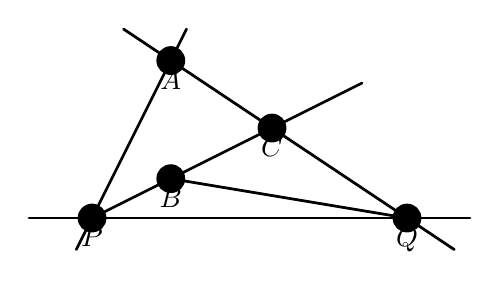
\begin{tikzpicture}
    \tkzSetUpPoint[shape=circle,size=10,color=black,fill=black]
    \tkzSetUpLine[line width=1]
    \tkzDefPoints{0/0/P, 4/0/Q, 1/0.5/B, 1/2/A}
    \tkzInterLL(P,B)(Q,A) \tkzGetPoint{C}

    \tkzDrawLine(P,A)
    \tkzDrawLine(Q,A)
    \tkzDrawLine(P,Q)
    \tkzDrawLine[add=0 and 0.5](P,C)
    \tkzDrawSegments(B,Q)

    \tkzDrawPoints(P,Q,B,C,A)
    \tkzLabelPoint[below](P){$P$}
    \tkzLabelPoint[below](Q){$Q$}
    \tkzLabelPoint[below](B){$B$}
    \tkzLabelPoint[below](C){$C$}
    \tkzLabelPoint[below](A){$A$}
\end{tikzpicture}
\end{document}
